\chapter{Estado del Arte}\label{chapter:state-of-the-art}

En el ámbito de la investigación sobre el crecimiento tumoral y la simulación de procesos biológicos, se han desarrollado diversas aproximaciones y modelos matemáticos que buscan comprender y representar con precisión la dinámica de las células en tejidos cancerosos. A continuación, se revisa el estado actual del arte en cuanto a modelos y técnicas utilizadas en este campo.

\section{Modelos clásicos de crecimiento tumoral}

Históricamente, diversos modelos clásicos han sido propuestos para describir el crecimiento tumoral. Entre ellos se destacan el modelo de crecimiento exponencial de Malthus, la ley de crecimiento de Gompertz y el modelo logístico de Verhulst \cite{viabarre2019}. Estos modelos han sido ampliamente estudiados y han servido como base para comprender el comportamiento básico de las poblaciones celulares en tumores.

\subsection{Ley de Malthus}

Uno de los más comunes experimentos en microbiología consiste en analizar el crecimiento de microorganismos unicelulares bajo ciertas condiciones, a lo largo de varios días. Se coloca una cantidad inicial de microorganismos dentro de un tubo de ensaye que contiene nutrientes. Después de este proceso de inoculación, a la colonia se le mantiene en condiciones que favorecen su crecimiento. Las bacterias se reproducen exitosamente al dividirse sustancialmente, tanto que su tamaño resulta incrementado radicalmente.

Consideremos a $N(t)$ la densidad de bacterias observada en el tiempo $t$. Si pudiéramos observar las divisiones celulares durante un determinado período de tiempo, nos percataríamos que se obtienen $k$ nuevas células. Así, $k$ es la razón de reproducción por unidad de tiempo. Si despreciamos la muerte celular que pudiera ocurrir en la colonia, obtenemos la relación fundamental de la densidad de bacterias dada por:

\begin{equation}
    \frac{dN}{dt} = kN,
\end{equation}

esta ecuaci\'on es conocida como Ley de Malthus, cuya soluci\'on est\'a dada por:
\begin{equation}
    N(t) = N_{0}e^{kt},
\end{equation}

donde $N_{0}$ es la poblaci\'on inicial de bacterias.

%(Aqui viene una imagen)
\begin{figure}[!ht]
\begin{center}
\scalebox{0.75}{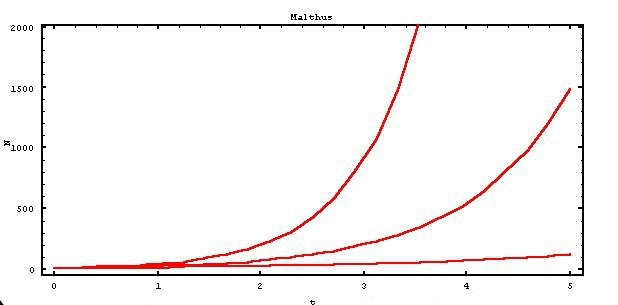
\includegraphics{img/fig-malthus.jpg}}
\end{center}\vspace*{-0.6cm}
\caption[Ley de Malthus]{La ecuación se basa en la idea de que la tasa de crecimiento de una población es proporcional a su tamaño actual. En otras palabras, cuanto mayor sea la población, más rápido crecerá.}
\label{fig-malthus}
\end{figure}

Claramente, este modelo tiene limitaciones insalvables, por lo que en principio no es una buena aproximación a la modelación de neoplasias, donde sí ocurren otros procesos adicionales (muerte, mecanismos de inhibición de crecimiento y propiedades físicas del medio que rodea a las células).

\subsection{Crecimiento logístico}
Consideremos la ley de Malthus de la sección anterior. Cabe la posibilidad de que la razón de crecimiento dependa directamente de los recursos disponibles de la población. Supongamos que la razón k de reproducción es simplemente proporcional a la concentración de nutriente C, esto es:
\begin{equation}
    K(C) = kC
\end{equation}

Supongamos también que unidades de nutriente son consumidas produciendo una unidad de incremento en la colonia. Esto implica que el crecimiento de bacterias y el consumo de nutrientes pueden ser descritos mediante las siguientes ecuaciones diferenciales ordinarias:
\begin{equation}
    \begin{split} % Esta ecuacion es (1)
        \frac{dN}{dt} = kN = kCN\\
        \frac{dC}{dt} = -\alpha N = -\alpha k CN
    \end{split}
\end{equation}
Tal sistema se resuelve de la siguiente manera:
\begin{equation}
    \begin{split}
        \frac{dC}{dt} = -\alpha \frac{dN}{dt}\\
        C(t) = -\alpha N(t) + C_{0}
    \end{split}
\end{equation}
 

$C_{0} = C(0) + \alpha N(0)$ es una constante. Si la población es inicialmente muy pequeña $C_{0}$ es aproximadamente igual a la cantidad de nutrientes en el tubo de ensayo. Substituyendo en relaci\'on de (1) obtenemos:
\begin{equation}
    \frac{dN}{dt} = k(C_{0} - \alpha N)N
\end{equation}
Este tipo de ley de crecimiento se conoce como crecimiento logístico. Comúnmente aparece en la forma:
\begin{equation}
    \frac{dN}{dt} = rN(1 - \frac{N}{B})
\end{equation}

La soluci\'on de la anterior ecuaci\'on es:
\begin{equation}
    N(t) = \frac{N_{0}B}{(N_{0} + (B - N_{0})e^{-rt})}
\end{equation}
% fotaca
%(Aqui viene una imagen)
\begin{figure}[!ht]
\begin{center}
\scalebox{0.75}{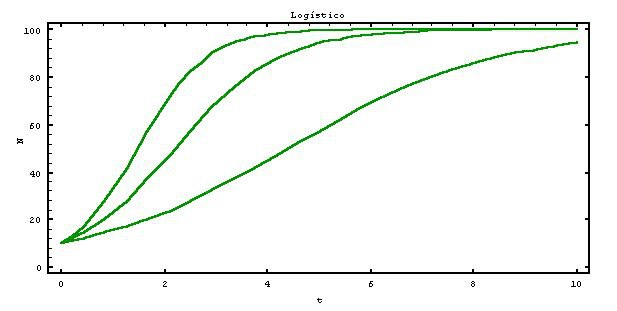
\includegraphics{img/fig-logistico.jpg}}
\end{center}\vspace*{-0.6cm}
\caption[Curva de crecimiento de Ley de Crecimiento Log\'istico]{Curva de crecimiento de Ley de Crecimiento Log\'istico}
\label{fig-logistico}
\end{figure}

\subsection{Ley de Gompertz}
La ley de Gompertz, es una de las principales leyes en la modelación de tumores sólidos y considera otras de las características de la tumoración:
\begin{itemize}
    \item el problema de las geometrías complicadas
    \item las células en el interior de un tumor no tienen acceso a nutrientes y oxígeno.
\end{itemize}

Estas se consideran en este modelo suponiendo que la razón de crecimiento declina tanto como la masa celular crece. Este modelo surge porque en muchos de los casos, el crecimiento puede ser verdaderamente complejo por lo que resultaría difícil predecir estados posteriores del crecimiento contando solo con pocas observaciones puntuales. La ley de Gompertz permite predicciones más o menos exactas, basadas en el sistema de ecuaciones diferenciales siguiente:
\begin{equation}
    \begin{split}
        \frac{dN}{dt} = k_{1}NG\\
        \frac{dG}{dt} = -k_{2}G,\label{eq-gompertz}
    \end{split}
\end{equation}

donde $k_{1} \geq O_{1}k_{2}$ son constantes, $N(t)$ es el vol\'umen del tumor al tiempo $t$ y $G(t)$ es una funci\'on enteramente descrita por la segunda ecuaci\'on. La expresión $k_{2}G$ puede pensarse como la fracción de $N(t)$ que se duplica en tamaño durante el instante $dt$. Lo que distingue a este modelo es que considera un mecanismo interno de autoinhibición que se intensifica tanto como se incrementa el crecimiento, resultando en un crecimiento exponencial de decrecimiento que alcanza un límite asintótico en el tamaño del tumor. La solución de ~\ref{eq-gompertz} es escrito en la forma:
\begin{equation}
    N(t) = N(0) \mathrm{e}^{(\frac{k_{1}}{k_{2}})G(0)(1 - \mathrm{e}^{-k_{2}t})}
\end{equation}

% fotaca
%(Aqui viene una imagen)
\begin{figure}[!ht]
\begin{center}
\scalebox{0.75}{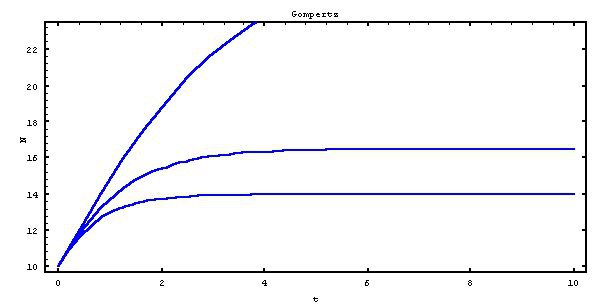
\includegraphics{img/fig-gompertz.jpg}}
\end{center}\vspace*{-0.6cm}
\caption[Curva de crecimiento de Ley de Gompertz]{Curva de crecimiento de Ley de Gompertz}
\label{fig-gompertz}
\end{figure}
\newpage

\subsection{Modelo logístico de Verhulst}
La ecuación Verhulst fue publicada por primera vez por Pierre François Verhulst en 1838 después de haber leído el \textit{Ensayo sobre el principio de población} de Thomas Malthus.

Verhulst derivó su ecuación logística para describir el crecimiento auto-limitado de una población biológica.

El crecimiento logístico está relacionado con el crecimiento exponencial, de hecho para pequeños valores de la magnitud que presenta el crecimiento logístico se asemeja mucho al crecimiento exponencial. Sin embargo, a partir de un cierto punto el crecimiento se ralentiza, eso hace que la curva pueda representar adecuadamente la propagación de rumores, la extensión de una innovación tecnológica o una epidemia: al principio estas se propagan rápidamente, cada ``infectado'' o ``afectado'' por la innovación es susceptible de traspasar el ``contagio'' a otro individuo que tenga contacto con él, pero cuando el número de ``infectados'' crece es más difícil encontrar una persona que previamente no haya estado en contacto con la enfermedad o innovación.

Esta típica aplicación de la ecuación logística es un modelo común del crecimiento poblacional según el cual:
\begin{itemize}
    \item la tasa de reproducción es proporcional a la población existente.
    \item la tasa de reproducción es proporcional a la cantidad de recursos disponibles.
\end{itemize}

El segundo término modela la competición por los recursos disponibles, que tiende a limitar el crecimiento poblacional.

Si $P$ representa el tamaño de la población y $t$ representa el tiempo, este modelo queda formalizado por la ecuación diferencial:
\begin{equation}
   \frac{dP}{dt} = rP(1 - \frac{P}{K})\label{eq-poblacion}
\end{equation}

donde la constante $r$ define la tasa de crecimiento y $K$ es la capacidad de persistencia. La soluci\'on general a ~\ref{eq-poblacion} es una funci\'on logística. Con una poblaci\'on inicial $P_{0}$:
\begin{equation}
    P(t) = \frac{KP_{0}e^{rt}}{K + P_{0}(e^{rt} - 1)}
 \end{equation}

donde 
\begin{equation}
    \lim_{t \to \infty} P(t) = K
\end{equation}

Investigaciones como las de \cite{book} comparan y relacionan estos modelos clásicos utilizando datos provenientes de sistemas de cultivo de esferoides tumorales multicelulares (MTS). Este tipo de estudios establece la relevancia y limitaciones de estos enfoques tradicionales.

\section{Enfoques basados en autómatas celulares}
Un autómata celular es un sistema dinámico discreto gobernado por reglas simples deterministas. En él se considera al espacio y al tiempo de manera discreta. El autómata consiste en una red uniforme y regular, cuyas posiciones se denominan sitio o ``célula''. Los primeros autómatas \cite{viabarre2019}, desarrollados por Von Neumann, datan de 1947. D\"uchiting y colaboradores proponen los primeros modelos computacionales basados en autómatas celulares aplicados a MTS. Estos autores modelan el crecimiento de un esferoide tumoral a partir de la proliferación de las células tumorales individuales que lo constituyen.

Un autómata celular se define a partir de una matriz ($n$ dimensional), la asignación de un conjunto de estados iniciales a cada autómata de la matriz, el conjunto de estados posibles de cada autómata, una función de transición que asigna un nuevo estado a un autómata teniendo en cuenta el estado de todos sus vecinos, una función que asigna a cada autómata el conjunto de sus vecinos (función de vecindad), una distribución de probabilidades para cada posición de la matriz y momento determinado, y un conjunto opcional de estados finales. Las posiciones dentro de la estructura regular están definidas por índices sobre los cuales es posible especificar las posiciones permitidas. De manera que las células, localizadas en una red espacial progresarán en su ciclo reproductivo y vital dependiendo de su acceso a los nutrientes. La división de una célula supondrá la necesidad de ubicarla en una nueva posición, mientras que la muerte de alguna de ellas puede hacerla desaparecer del agregado celular y generar el movimiento de las células que la rodean.

Los autómatas celulares han demostrado ser herramientas poderosas para simular el crecimiento tumoral. Investigadores han utilizado autómatas celulares para modelar diversas etapas del desarrollo tumoral, incluyendo la etapa avascular [\cite{dormann},\cite{kansal2}], la invasión celular \cite{rejniak}, y las interacciones complejas con el entorno \cite{rejniak}.

En \cite{ruanxiaoca}, se presenta un modelo que simula el crecimiento tumoral, considerando las interacciones entre células cancerígenas, células normales y el sistema inmunológico. La flexibilidad de los autómatas celulares permite capturar la dinámica compleja de sistemas biológicos con un alto grado de realismo.

\section{Modelado con mecánica de medios continuos (MMC)}
La mecánica de medios continuos (MMC) es la rama de la Mecánica que propone un modelo unificado para sólidos deformables, sólidos rígidos y fluidos (líquidos y gases), basado en la hipótesis fundamental de la continuidad del medio: se supone la materia distribuida de forma continua en cualquier porción de volumen que se considere. El término medio continuo se usa tanto para designar un modelo matemático, así como cualquier porción de material cuyo comportamiento se puede describir adecuadamente por ese modelo.

El enfoque de MMC ha sido utilizado para modelar el crecimiento tumoral desde una perspectiva de variables continuas. En \cite{ariel} se presenta un modelo que utiliza ecuaciones constitutivas y leyes de balance para describir la evolución del tumor en términos de masa y energía. Este enfoque proporciona una representación detallada de los procesos físicos involucrados en el desarrollo tumoral.

Otros estudios, como los de \cite{preziosi} y \cite{preziosi2}, han considerado la tensión ideal en todas las células del organismo, proponiendo que la aparición de un tumor se interpreta como una falla en los mecanismos de homeostasis.

\section{Avances recientes y terapias innovadoras}

En la actualidad, los avances en el tratamiento del cáncer han introducido terapias más precisas y menos invasivas. La terapia dirigida, que interfiere con moléculas específicas que promueven el crecimiento canceroso, y la inmunoterapia, que potencia la respuesta inmune del cuerpo, se presentan como metodologías prometedoras \cite{soerjomataram2020}\cite{seke2021}.

Algunos de los avances más prometedores:
\begin{itemize}
    \item \textbf{La terapia celular personalizada} o \textbf{terapia dirigida} es un enfoque innovador para tratar el cáncer que utiliza células inmunitarias del propio paciente para combatir la enfermedad. Los médicos extraen células inmunitarias, las cultivan en el laboratorio y luego las modifican para que sean más efectivas contra el cáncer. Luego, estas células modificadas se infunden de nuevo en el paciente para ayudar a combatirlo. Hasta ahora muy pocas personas han sido tratadas con este tipo de medicamentos, pero sus avances recientes muestran que podría sustituir algunos de los tratamientos que se utilizan ahora, como la cirugía, quimioterapia, radioterapia o terapia hormonal.
    \item \textbf{La terapia génica} es un enfoque relativamente nuevo en la investigación que utiliza la manipulación genética para tratar el cáncer. En este enfoque, los médicos insertan material genético en células para corregir mutaciones que lo causan. También se puede usar para enseñar al sistema inmunitario a reconocer y atacar células cancerígenas o viceversa, adem\'as de proteger las células sanas. Esto puede ayudar a prevenir la progresión del cáncer y mejorar el pronóstico del paciente.
    \item \textbf{La radioterapia de haz estrecho} es una forma avanzada de radioterapia que utiliza tecnología sofisticada para dirigir un haz de radiación con mayor precisión a las áreas afectadas. Esto permite a los médicos tratar el cáncer con una dosis más alta de radiación, lo que puede mejorar los resultados del tratamiento y también reducir el número de sesiones necesarias o la longitud del tratamiento.
    \item \textbf{Las vacunas terapéuticas} son una de los más recientes descubrimientos en el campo de esta enfermedad, que utiliza las propias defensas del sistema inmunológico del cuerpo para combatir la enfermedad. Los médicos crean una vacuna personalizada para cada paciente que ayuda a estimular el sistema inmunológico para combatir el cáncer. Pero en el caso del cáncer, a diferencia de las bacterias y virus, sus células se parecen más a nuestras células sanas y normales, por lo que es más complicado generar vacunas eficaces. Además, cada tumor es en cierto modo único y requiere sus propios antígenos distintivos. En lo que también ha habido un avance importante en los últimos años son las vacunas preventivas, que han sido recientemente aprobadas por la Administración de Alimentos y Medicamentos(FDA) de los EE. UU.
\end{itemize}

La investigación se centra en estrategias terapéuticas más efectivas, incluyendo la expresión de genes proapopt\'oticos y quimiosensibilizadores, así como el silenciamiento dirigido de oncogenes \cite{seke2021}.

\section{Visualización tridimensional y técnicas de Renderización}

La representación visual tridimensional del crecimiento tumoral es esencial para comprender cómo afecta a los tejidos circundantes. La técnica de Marching Cubes \cite{lorensen1987} se ha utilizado para la renderización en 3D de tumores, proporcionando visualizaciones detalladas. La visualización tridimensional es crucial para médicos y científicos, ya que permite una mejor comprensión de la evolución del tumor y su impacto en el entorno.

\section{Contribuciones de la investigación propuesta}

La investigación propuesta busca avanzar en la simulación integral del crecimiento tumoral, abordando tanto las etapas avascular como vascular, así como procesos de invasión, migración y metástasis. La implementación de un autómata celular basado en una red de mundo pequeño \cite{watts} aporta flexibilidad y adaptabilidad a la simulación.

El enfoque dinámico de parámetros y factores en la simulación, junto con algoritmos eficientes para el procesamiento de grandes cantidades de células, constituyen contribuciones significativas. La visualización tridimensional mediante la técnica de Marching Cubes proporcionará una comprensión detallada del crecimiento tumoral, crucial para el desarrollo de terapias y tratamientos efectivos.

En resumen, el estado del arte en este campo refleja una combinación de enfoques clásicos y contemporáneos, destacando la importancia de modelos como los autómatas celulares y la visualización tridimensional para comprender y abordar el crecimiento tumoral desde diversas perspectivas. La investigación propuesta se posiciona como un avance significativo al integrar estos enfoques y contribuir con herramientas más flexibles y efectivas para la simulación y visualización del desarrollo tumoral.